\documentclass{article}
\usepackage{amsmath}
\usepackage{amssymb}
\usepackage{enumerate}
\usepackage{tikz}

\title{MAT -- 112: Calculus I and Modeling\\
\large{Solution 1}}
\author{Thomas R. Cameron}
\date{1/26/2018}

\begin{document}
\maketitle

\subsection*{Other Problems}

\paragraph*{Problem 1.} By definition, two lines $\mathcal{L}_{1}$ and $\mathcal{L}_{2}$ are perpendicular if $\mathcal{L}_{1}$ is horizontal and $\mathcal{L}_{2}$ is vertical, or the slope of $\mathcal{L}_{1}$ is $m\neq 0$, and the slope of $\mathcal{L}_{2}$ is $-\frac{1}{m}$. The horizontal and verticle case is clear, since the intersection of the two lines creates a right angle (side of a square) as seen below.
\begin{figure}[h]
\centering
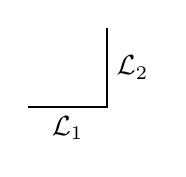
\begin{tikzpicture}
\path[draw] (0,0) -- node[below] {$\mathcal{L}_{1}$} (1,0) -- node[right] {$\mathcal{L}_{2}$} (1,1);
\end{tikzpicture}
\end{figure}


The case where $\mathcal{L}_{1}$ has a slope of $m\neq 0$ and $\mathcal{L}_{2}$ has a slope of $-\frac{1}{m}$ is shown below. Starting at the point $(x,y)$, the line $\mathcal{L}_{1}$ denotes going over $1$ and up $m$, whereas the line $\mathcal{L}_{2}$ denotes going over $1$ and down $\frac{1}{m}$. 
\begin{figure}[h]
\centering
\begin{tikzpicture}[scale=1.3]
\draw[gray] node[black,left] {$(x,y)$} (0,0) -- node[black,above] {$1$} (1,0);
\draw[dashed] (1,0) -- node[right] {$m$}(1,2);
\draw[blue,dashed] (0,0) -- node[black,left] {$\mathcal{L}_{1}$}(1,2);
\draw[dashed] (1,0) -- node[right] {$-\frac{1}{m}$}(1,-0.5);
\draw[green,dashed] (0,0) -- node[black,below] {$\mathcal{L}_{2}$}(1,-0.5);
\end{tikzpicture}
\end{figure}
~\\
In order to show that the angle of intersection is a $90$ degree angle, we can show that the triangle outlined by the blue, green, and black dashed lines is a right triangle. Note that the both smaller triangles must be right triangles, since one of their angles is the intersection of a horizontal and vertical line. Therefore, the length of the blue dashed line is $\sqrt{1+m^{2}}$ and the length of the green dashed line is $\sqrt{1+1/m^{2}}$. Furthermore, note that
\[
\sqrt{(1+m^{2})+(1+1/m^{2})}=\sqrt{(m+1/m)^{2}}=m+1/m
\]
which is the length of the black dashed line. It follows that the triangle is outlined by the blue, green, and black dashed lines is a right triangle. 


\paragraph*{Problem 2.} To show that $h=g\circ f$ is a function from  $A$ to $C$, we must show that $h$ takes each element of $A$ to exactly one element of $C$. To this end, let $\alpha$ be an element of $A$. Then, $f(\alpha)$ is a unique element in $B$, which is the domain of the function $g$. It follows that $g$ takes $f(\alpha)$ to exactly one element of $C$. Therefore, $h(\alpha)=g(f(\alpha))$ is a unique element in $C$. 

\paragraph*{Problem 3.} Using the method of completing the square, we can transfer the quadratic $ax^{2}+bx+c$, where $a\neq 0$, into vertex form as follows
\begin{align*}
ax^{2}+bx+c&=a\left(x^{2}+\frac{b}{a}x\right)+c \\
&=a\left(x^{2}+\frac{b}{a}x+\frac{b^{2}}{4a^{2}}\right)+c-\frac{b^{2}}{4a} \\
&=a\left(x+\frac{b}{2a}\right)^{2}+\frac{4ac-b^{2}}{4a}
\end{align*}
Once in vertex form, we can identify the vertex, axis of symmetry, $x$-intercept, and $y$-intercept.\\
\emph{Vertex:}	$(-\frac{b}{2a},\frac{4ac-b^{2}}{4a})$\\
\emph{Axis of Symmetry:}	$x=-\frac{b}{2a}$\\
\emph{y-intercept:} $(0,c)$ \\
\emph{x-intercept:}	The $x$-intercepts occur when the quadratic equals zero. Thus, we can solve for $x$ as follows
\begin{align*}
a\left(x+\frac{b}{2a}\right)^{2}+\frac{4ac-b^{2}}{4a}&=0 \\
a\left(x+\frac{b}{2a}\right)^{2}&=\frac{b^{2}-4ac}{4a} \\
\left(x+\frac{b}{2a}\right)^{2}&=\frac{b^{2}-4ac}{4a^{2}} \\
x+\frac{b}{2a}&=\pm\frac{\sqrt{b^{2}-4ac}}{2a} \\
x&=-\frac{b}{2a}\pm\frac{\sqrt{b^{2}-4ac}}{2a}
\end{align*}
Note that we have derived the quadratic formula.

\end{document}